\documentclass[12pt, a4paper, openany, twoside]{book}
\usepackage[italian]{babel}
\usepackage[T1]{fontenc}
\usepackage[utf8]{inputenc}
\usepackage{amsmath} 
\usepackage{xcolor}
\usepackage[margin=1in]{geometry}
\usepackage{hyperref}
\usepackage{graphicx}
\graphicspath{{./img/}}
\usepackage{tikz}
\hypersetup{
    colorlinks=true,
    linkcolor=blue,
    filecolor=magenta,      
    urlcolor=cyan,
}
%usepackage[latin1]{inputenc}
\begin{document}
\fontfamily{cmss}\selectfont
\pagestyle{plain}
\author{DaveRhapsody}
\title {Basi di Dati}
\date {4 Marzo 2020}
\maketitle
\tableofcontents
\chapter*{Introduzione}
Un database, o base di dati, o db (che scriverò d'ora in poi) è un insieme di 
dati, tipo deposito, per qualsiasi genere di uso, sia aziendale, che personale.
I suddetti dati sono inseriti, letti, e soprattutto \underline{organizzati} 
secondo certe regole.
\paragraph{Alcuni esempi: }
\begin{itemize}
	\item Agende telefoniche
	\item Studenti di una classe o scuola
	\item Qualsiasi insieme generico in cui ogni elemento differisce da un altro
	secondo delle linee guide (campi) che si decidono alla base.
\end{itemize}
Da Linguaggi di Programmazione sono state viste le Struct, o Record, che sono
delle strutture per i dati statiche, concrete ed eterogenee, aventi più campi
non necessariamente dello stesso tipo. \\ \\
Bene, un DB è un array di record, in cui bisogna garantire integrita, consistenza
e NON ridondanza dei dati.
\section{Interazione tra campi}
Tra loro i campi di questi record possono interagire, nel senso che partendo dal
valore di un determinato campo, si può ricavare il valore di un altro campo.
Esempio? Il \underline{codice fiscale}, che è ricavato da una formula che non 
ricordo mai nella vita forever MA prendendo come dati il nostro nome, cognome, 
etc.
\paragraph{Questo sarà un campo calcolato}
\section{Dove si colloca un DB?}
\begin{itemize}
	\item Intefaccia utente
	\item Applicativi
	\item Software di ambiente e di sistema
	\item DB
	\item Sistema operativo
	\item Hardware
	\item Sistema di comunicazione di rete
\end{itemize}
Impropriamente si può definire nel mezzo
\section{Problemi da NON avere}
\begin{itemize}
	\item Ridondanza dei dati: non devono esserci dati ripetuti, ogni record è
	U N I V O C O. Per renderlo tale credo nel corso che vedremo come si fa, 
	spoiler: chiavi, la nostra futura bacinella di bestemmie.
	\item Rischi di incoerenza: i dati devono essere consistenti, ossia dato un
	valore, se lo si attribuisce ad un simbolo (dato, variabile, campo), quel
	valore dovrà essere SEMPRE quello, per ogni volta che si richiama quel 
	simbolo
\end{itemize}
\section{Condivisione dei dati}
Data un'organizzazione avente più dipendenti, è naturale che la suddetta possa
condividere un determinato insieme di dati, infatti ad ogni settore corrisponde
un sistema informativo (Per chi ha fatto economia, il SIA).\\ \\
Cosa accade quando si condivide una risorsa? Esatto, bisogna fare in modo che
non avvengano accessi concorrenti, quindi sono implementate funzioni e 
procedure di prevenzione di questo genere di problemi. Un DB non protetto da
modifiche NON consentite, oltre a fare schifo tipo fortissimo forever maonna guarda
da bruciarlo, è NON integro. 
\paragraph{Un DB deve essere integro}
\chapter{DBMS}
Il DBMS (Database Management System) è un software in grado di gestire i 
DB.. E grazie al piffero direi, ma perchè si usa? Perchè un DB è una risorsa
condivisa, e siccome potrebbe contenere dati importanti, serve un software che
consenta di tenerla pulita e integra.
\section{Cosa gestiscono}
Le moli di dati su cui operano i DBMS sono tendenzialmente di grandi dimensioni,
persistenti (con periodo di vita indipendenti dalle singole esecuzioni dei 
programmi che ci lavorano) e condivise, nel senso che diverse applicazioni ci 
possono lavorare sopra.
\section{Cosa devono garantire}
Dalle slides si riportano queste 3 qualità:
\begin{itemize}
	\item Affidabilità
	\item Sicurezza
	\item Effiecienza
\end{itemize}
E tra l'altro bastava anche solo specificare consistenza ed integrità, ma il 
ci siamo intesi
\section{Concetti fondamentali}
\subsection{Schema}
Lo schema è la descrizione dei campi di una tabella (banalmente, è come una 
classe in Java)
\subsection{Istanza}
L'istanza è un record allocato a cui assegno un valore per ogni campo (in Java
erano gli oggetti)
\subsection{Modello}
Il modello è l'insieme dei vari costrutti (o regole) utilizzati per organizzare
i dati e descriverne i cambiamenti nel tempo. 
\paragraph{Cosa compone un modello}
Le strutture di rappresentazione dei dati: Nel nostro caso si analizzerà 
la relazione. In base alla struttura cambia il modello, ad esempio il modello
\textbf{relazionale} userà la relazione, mentre il modello a oggetti ad esempio
userà altre strutture.
\subsection{Tipo di modello}
Ce ne sono due:
\paragraph{Logico:} Vengono utilizzati dai programmi e non dipendono
dalle strutture fisiche. Esempio: Relazionale, reticolare, etc.
\paragraph{Concettuale:} Sono ancora più in alto del modello logico,
quindi sono anche indipendenti dal DBMS, e sono delle descrizioni del mondo
reale, usati in fase di progettazione (Quando studieremo il modello E-R 
partiranno le imprecazioni)
\section{Architettura dei DBMS}
Tra un BD e L'udente (o i programmi) ci sono due schemi, schema fisico e schema
logico. Lo schema fisico è vicino al DB mentre il logico all'utente. (Quando 
verrà detto Utente, si intende sia Umano che Programma).
\subsection{Schemi}
Come menzionato prima ci sono schema fisico e logico, il fisico è banalmente
la reppresentazione di files, blocchi di memoria, cache etc. mentre il logico
è quello che abbiam visto prima, quindi schema relazionale etc.
\subsection{Indipendenza dei dati}
Il livello logico è indipendente dal fisico, nel senso che se tu hai un record
avente dentro un ID e altri due campi, ti importa poco se verrà salvata su un
SSD o su un floppy disk di fine 1800, sempre un record dovrai avere.
\paragraph{Osservazione:} Prendiamo l'ipotesi di un record avente id e numero
di telefono. (Non l'ho specificato ma l'ID è un campo numerico intero 
che identifica univocamente il record, fine) Se volessimo in modo sadico dividere
il numero in prefisso + numero? Esatto, cambia lo schema logico, ed il record
passa da 2 a 3 campi.
\paragraph{E lo schema fisico?} Dalle slide non si capisce, quindi azzardo una
risposta: siccome lo schema logico è indipendente dal fisico, non dovrebbe
cambiare.. Ma non ne son sicuro.
\subsection{Le viste}
Se l'utente accedesse di cattiveria direttamente allo schema logico, ad ogni
cambiamento allora dovrebbe cambiare tutto il suo programma. Come si risolve?
Con le viste (O schemi esterni) che sono dei sottoinsiemi dello schema logico,
che quindi contengono quantità di dati limitate (allo scopo di quell'applicativo).
\paragraph{In che senso?} Se l'utente è la portineria, gli si crea una vista
avente dati legati alla portineria.
E sì, schema logico ed esterno sono indipendenti dal fisico, questo significa
che l'applicativo non cambierà se cambio il supporto fisico su cui ho messo il
DB. E addirittura il livello esterno è indipendente dal logico.
\subsection{Linguaggi del DBMS}
Ce ne sono due, uno è un linguaggio descrittivo dei dati, e l'altro è di 
manipolazione (sql). Uno descrive le strutture, l'altro ci scrive dentro e 
legge.
\chapter{Modello Entità-Relazione}
Il modello E-R è uno schema concettuale che consente di rappresentare la 
realtà tramite entità e relazioni tra esse.
\section{Concetto di entità}
E' un'astrazione di un certo insieme di dati (come le classi in Java). Graficamente
un'entità è rappresentata da un rettangolo con all'interno il nome dell'entità.
\paragraph{Il nome dev'essere descrittivo},
ad ogni entità inoltre occorre dare una definizione. Del tipo Automobile, è 
quell'oggetto che se è colorato di rosso ed ha un V8 sotto il cofano ti permette
di avere orgasmi multipli (dai che mi volete bene, lo so <3).
\paragraph{L'istanza di un'entità è il caso specifico:} Automobile = entità, 
Bmw, Ferrari, Porsche è l'istanza. Il nome che identifica un'entità deve essere
singolare ed espressivo, no abbreviazioni, no codici.
\section{Attributo dell'entità}
E' una proprità, o meglio, un campo del record che serve ai fini dell'applicazione
, questo valore dipende solo dall'istanza dell'entità, non dipende da altri
elementi nello schema. Inoltre ogni attributo ha un intervallo di valori finito.
(Il concetto di infinito in informatica non esiste se non per le mie funzioni
ricorsive rottissime di Prolog e Lisp) 
\paragraph{Reppresentazione:}
\begin{center}
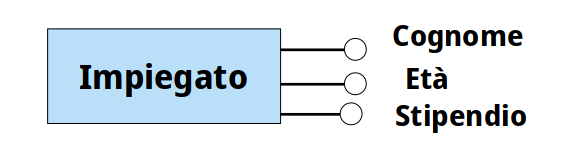
\includegraphics[width=0.75\textwidth]{2.png}
\end{center}
Se il campo è chiave, il pallino diventa pieno. (Sto odiando questa slide, è 
tutto così non simmetrico che sclero)
\section{Le Relazioni}
Una relazione (o associazione) è un legame logico tra più entità, ed il numero
di esse determina il grado (numero di entità obv), si rappresenta con un rombo
e dentro ci si scrive cosa lega le entità. Come in questo esempio:
\begin{center}
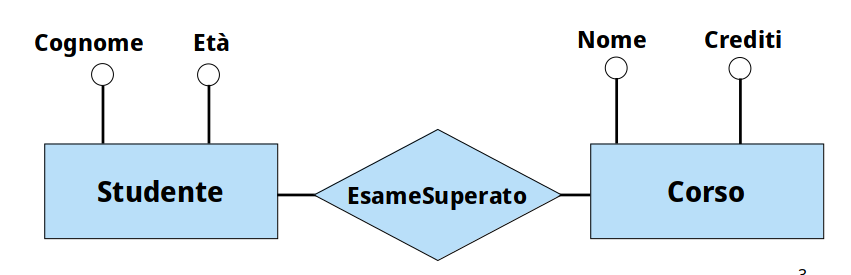
\includegraphics[width=0.75\textwidth]{3.png}
\end{center}
Siccome c'è differenza tra queste relazioni e le relazioni del modello relazionale,
per comodità le chiamerò associazioni. Quindi associazioni -> modello e-r, relazioni ->
modello relazionale.
\paragraph{Come scrivere le associazioni:} Bisogna usare dei sostantivi al 
singolare. Come da esempio: Se ho due entità studente ed esame ed in mezzo ci
metto "Supera" è sbagliato. Si deve mettere "Esame superato". (Alle superiori
ero abituato che il verbo andasse all'infinito, che ha più senso ed è più 
leggibile, ma icchè vi devo dì, noi s'attacca l'asino indoe vuole i' padrone).
\paragraph{Tra due entità posso insierire più associazioni:} Ad esempio prendendo
uno studente ed un corso, ci puoi applicare due associazioni, una può essere
"frequenZa" e l'altra boh.. "Frequenza passata". E da notare che nelle slides 
ha messo "Frequenta" e "Frequentato in passato".. Niente verbi, ovvio.
\paragraph{Anche un'associazione può avere degli attributi:} E' una proprietà
\textbf{locale} che serve ai fini dell'utente, non è una proprietà della singola
entità ma di tutte coloro che sono in legame.
\paragraph{In termini umani:} E' una funzione che associa ad ogni istanza di 
quella associazione un valore che appartiene ad un dominio dell'attributo.
\paragraph{Esempio:} Studente - \underline{superamento} - Esame, un attributo
di superamento potrebbe essere Voto. (Tra l'altro lui ha messo esameSuperato.. 
boh, diobono ok che superato è un aggettivo, ma è participio passato di superare,
queste slides sono un casino).
\section{Vincoli di cardinalità}
La cardinalità di una realzione specifica le quantità di interazione di istanze
di più entità in un'associazione. si specifica un valore minimo ed uno massimo.
Quindi è un dominio, un insieme finito di valori che è possibile assumere.
\paragraph{Definizione:} Un vincolo di cardinalità è un limite di istanze di
una associazione a cui può partecipre un'istanza di una o più entità, caratterizza
meglio il significato di una associazione.
\paragraph{Esempio banale babbarello:} Studente - \underline{Frequenza} - Corso,
Da 0 a N studenti frequentano N corsi. 1 corso può essere frequentato da N
studenti. 1 studente frequenta N corsi.
\section{Tipi di assoiazione}
Rimanendo nel contesto delle relazioni binarie, ci sono 3 tipi di relazione:
\begin{enumerate}
	\item Relazione uno a uno
	\item Uno a Molti
	\item Molti a Molti
\end{enumerate}
Le quali si spiegano da sole, non c'è molto da specificare.
\section{Generalizzazioni e Relazioni Is-A}
Partendo dall'Is-A
\subsection{Relazione IS-A}
E' una relazione che introduce il fatto che un'istanza possa appartenere a più
entità, esempio Pilota, Pilota di Rally. E' anche definita relazione di sottoinsieme,
e si utilizza per entità in cui una sia sottoinsieme dell'altra, o meglio. Una 
deve essere "padre" dell'altra, che si chiamerà "figlia".
\paragraph{Esempio:} Fuoristrada \underline{Is-A} Automobile \underline{Is-A} Veicolo
\paragraph{Principio di ereditarietà:} Ogni attributo e proprietà dell'entità
padre è anche proprietà della sua sottoentità, va da sè che la figlia può avere
anche le sue proprietà. (Oh è come le classi di Java, funziona tutto così)
\paragraph{Graficamente:}
\begin{center}
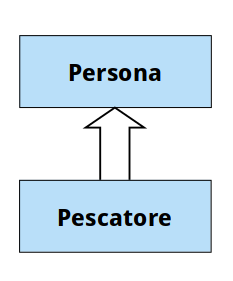
\includegraphics[width=0.75\textwidth]{4.png}
\end{center}
\subsection{Generalizzazione tra entità}
Hai un'entità padre ed una serie di figlie, quello che fai è con un arco unirle,
fine. 
\begin{center}
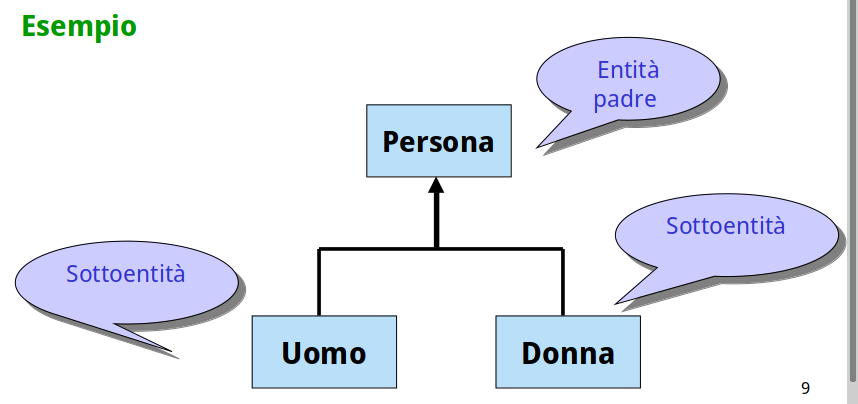
\includegraphics[width=0.75\textwidth]{5.png}
\end{center}
Una generalizzazione può essere di due tipi:
\begin{itemize}
	\item Completa: L'unione delle istanze delle sottoentità è uguale all'insieme
	delle istanza del padre
	\item Non completa: in cui questo non accade
\end{itemize}
\paragraph{Spiegato meglioglioglio:} Hai uomo e donna, e poi essere umano, se prendi
tutti gli uomini + tutte le donne e fai un insieme contenente tutti essi, ottieni
l'essere umano. (Sì, LGBT, abbiate pietà, non è il momento di polemizzare) \\
Ipotizziamo gli animali: hai cane gatto e criceto, e poi animali.. Beh se sommi
tutti i gatti criceti e cani, non ottieni l'insieme degli animali. Mancano i
gamberetti per esempio.
\paragraph{Detto scientificamente accurato:} Se le sotto entità sono partizioni
dell'entità padre, è completa, altrimenti no.
\paragraph{L'entità padre può avere più generalizzazioni}
\section{Attributi composti} Un attributo può esser definito su un dominio di più
campi. In altri termini, un attributo può essere a sua volta un record. Tipo
indirizzo (composto da via numero e cap), è uno di questi. Potrebbe essere anche
un attributo del tipo "dati anagrafici". Quando si ha questa situazione l'attributo
è composto.
\section{Relazioni n-arie}
La relazione BI-naria coinvolge due entità, la ternaria tre, la quaternaria.. 
Via, si è capito, se è n-aria coinvolge n entità. A sua volta anche la relazione
può avere i suoi attributi.
\paragraph{Esistono anche relazioni ricorsive o definite su se stesse:} Il classico
esempio è il papa. papa - \underline{successione} - papa, per tenervelo in testa
pensate a "Morto un papa, se ne fa n'altro".
\section{Identificatori/Chiavi}
E' un insieme di attributi o relazioni che ti permettono di identificare le
istanze di un'entità. (Per chi ha già fatto sta roba sono le chiavi primarie).
Ogni entità ha un certo insieme di identificatori (Da 1 a $\infty$, basta che
ce ne sia uno $\forall$ entità)
\subsection{Tipi di identificatore/chiave}
\begin{itemize}
	\item \textbf{Interno}: Formati solo da attributi dell'entità stessa. può 
	essere solo uno, possono essere anche più di uno. Come in questo esempio:
	\begin{center}
	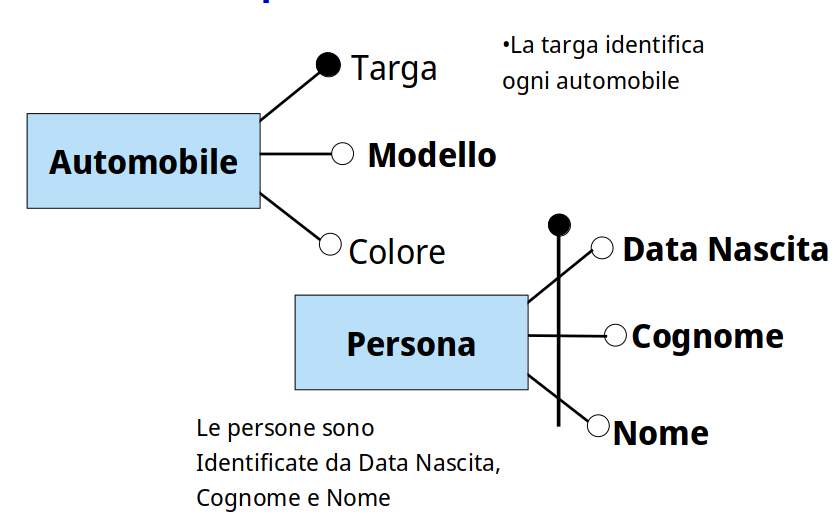
\includegraphics[width=0.75\textwidth]{6.png}
	\end{center}

	\item \textbf{Esterno}: E' formato da attributi dell'entità e da relazioni
	che la coinvolgono, oppure solo da queste relazioni.
	\paragraph{Esempio grafico:}
	\begin{center}
	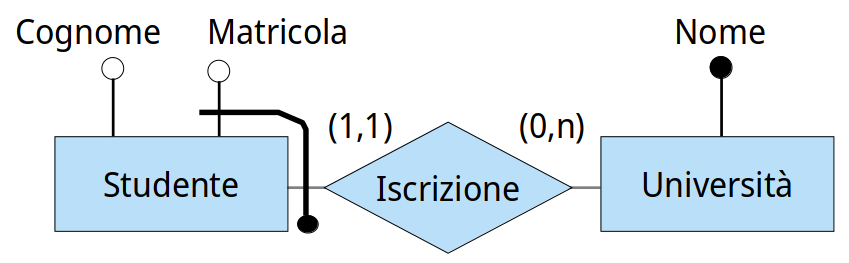
\includegraphics[width=0.75\textwidth]{7.png}
	\end{center}
\end{itemize}
\chapter{Livello logico}
Il livello logico è quello in cui figurano le strutture di rappresentazione 
logica dei dati. In altri termini, dove c'è uno schema logico che descrive una
realtà di interesse. E già qua occhio, non è uno schema concettuale come l'E-R,
qua non si parla di generalizzazione della realtà, ma di schema logico dei dati. 
\section{Modello relazionale}
Il concetto di relazione è da considerarsi in 3 modi diversi:
\begin{enumerate}
	\item Relationship (Associazione, classe di fatti)
	\item Relazione matematica (Qualunque sottoinsieme del prodotto cartesiano 
	blablabla)
	\item Relazione secondo il modello relazionale
\end{enumerate}
(Non mi soffermerò sulla spiegazione della relazione matematica, tenete solo
a mente che le n-uple al loro interno sono orninate e che tra le n-uple non c'è
ordinamento. Se volet buttateci dentro anche che ogni n-upla è univoca)
\subsection{Definizioni base}
\begin{itemize}
	\item \textbf{Struttura non posizionale}: Per ogni dominio si associa un attributo
	che ne descriva il ruolo
	\item \textbf{Relazione (o Tabelle)}: Letteralmente la rappresentazione
	matematica di una relazione in cui i valori per ogni colonna sono dello
	stesso tipo, e le righe sono diverse. In termini leggibili? Un cazzo di array 
	di record, con tutte le conseguenze che ne derivano.
	\paragraph{Osservazione:} Si è specificato "valori" per ogni colonna, NON a
	caso, perchè nel relazionale ci si basa su valori, ed i riferimenti tra i 
	dati in relazioni diverse sono rapprentati con valori dei domini che 
	compaiono nelle n-uple.
	\paragraph{La domanda è: Per quale f* motivo?} Le ragioni sono 3:
	\begin{enumerate}
		\item L'utente finale vede gli stessi dati dei programmatori, costituiti
		da tabelle
		\item L'indipendenza della rappresentazione delle strutture fisiche, 
		che cambiano in modo indipendente, quindi potete usare i floppyni del
		Nintendo o un SSD Nvme, I N D I P E N D E N Z A.
		\item i dati sono trasportabili da un sistema ad un altro per la ragione
		del punto 2
	\end{enumerate}
	\item \textbf{Schema di relazione}:
	\[
		nomeRelazione(Attributo_{1}, Attributo_{2}, Attributo_{n})
	\]	
	Facciamo che da ora nomeRelazione $\to$ nR e Attributo $\to$ A
	\item \textbf{Schema di Base di Dati}:
	\[
		superRelazione = \{nR_{1}(A_{1}, nR_{2}(A_{2}, ..., nR_{n}(A_{n}, )\}
	\]
	\item \textbf{N-upla}: Funzione che associa ad un certo insieme X di attributi,
	$\forall$ attributo A $\in$ X uno ed un solo valore del dominio di A
	\item \textbf{Istanza di relazione}: Data nR(A), l'istanza è l'insieme r di
	n-uple su nR
	\item \textbf{Istanza di Base di Dati}: Stesso identico concetto ma applicato
	allo schema della base di dati. Dato lo schema di prima (superRelazione),
	l'istanza è l'insieme delle relazioni r
	\item \textbf{Valori nulli}: Quando un VALORE non c'è in una determinata
	colonna, viene considerao Null 
\end{itemize}
\section{Strutture nidificate}
La realtà è rappresentabile con infiniti schemi equivalenti, nel \textbf{contenuto
informativo}. Ciò vuol dire che schemi equivalenti forniscono lo stesso
insieme di informazioni.
\paragraph{Premessa:} immaginatevi di volere rappresentare tutti gli scontrini di
un ristorante in cui ogni ricevuta ha come campi: \{Numero ricevuta, data emissione
e le varie voci di costo\}
\subparagraph{Le voci di costo:} Per ogni voce c'è una corrispondenza con un 
gruppo di portate, e per ciascun gruppo, il numero di porrtate e il costo del gruppo 
di portate, infine il totale.\\
Con un semplice schema ad elenco si ottiene alla fine la suddivisione in sezioni,
sottosezioni etc., riscrivendolo così vien fuori:
\begin{enumerate}
	\item Numero ricevuta
	\item Data Emissione
	\item Voci di costo
	\begin{enumerate}
		\item Gruppo di portate
		\begin{enumerate}
			\item Numero di portate
			\item Costo del gruppo di portate
		\end{enumerate}
	\end{enumerate}
	\item Totale speso
\end{enumerate}
\section{Vincoli}
Può accadere che dei DB siano sintatticamente corretti MA non rappresentano degli
stati realmente possibili nella realtà, ad esempio il 27 e lode (esempio delle
slides).
\paragraph{Risoluzione:} Per risolvere questo inconveniente occorre aggiungere
un vincolo che dica SE è 30 allora può avere lode, altrimenti non può. (Lode
può essere benissimo un campo booleano).
\section{Vincolo di integrità}
E' una proprietà che hanno i DB che va soddisfatta da tutte le istanze di uno
schema, le quali rappresentano informazioni corrette, consistenti, integre per
l'applicazione.
\paragraph{Banalmente:} E' una funzione booleana (O predicato for those who 
love Prolog) che per ogni istanza r dà:
\begin{itemize}
	\item \textbf{TRUE}: se l'istanza rappresenta la realtà
	\item \textbf{FALSE}: In caso contrario
\end{itemize}
\paragraph{A che servono?} Permettono di rappresentare in modo più preciso la
realtà, e quindi contribuiscono ad avere dati più consistenti. Inoltre sono
utili per progettare perchè lo schema risulta qualitativamente migliore
\subparagraph{Tipi di vincolo}
\paragraph{Vincolo intrarelazionale:} Definito all'interno della relazione.
Sono vincoli applicati agli \textbf{attributi} (si definiscono anche vincoli
di \textbf{dominio}), oppure vincoli di n-upla, o comunque relativi all'insieme
di n-uple di una relazione $\to$ Vincoli di relazione
\paragraph{Interrelazionale:} Definiti tra più relazioni
\section{Vincolo di n-upla}
Esprime condizioni sui valori di ciascuna n-upla in una relazione, ad esempio
non puoi avere due giocatori in una squadra con stesso numero di maglia.
\subparagraph{Sintassi}
\begin{itemize}
		\item Esressioni booleane (AND, OR, NOT)
		\item Atomi da confrontare (>,<, >= etc.)
\end{itemize}	
Per calcolare il valore di verità di un vincolo in una n-upla, occorre sostituire
i valori degli attributi nella n-upla, e poi calcolare il valore vero o falso.
\section{Vincolo di chiave}
C'è bisogno di individuare le informazioni che permettono di rappresentare ogni
oggetto di interesse con una n-upla differente e identificarlo nel caso in
cui ne abbia necessità.
\subsection{Cos'è una chiave} E' un insieme di attributi che identificano in modo
univoco le n-uple di una relazione. 
Un insieme K di attributi è \textbf{superchiave} per una relazione r se r non 
contiene due n-uple distinte $t_{1}$ e $t_{2}$ con $t_{1}[K]$ = $t_{2}[K]$.
\\ Una chiave tipica è il numero di matricola, che identifica uno studente, e
siccome è un solo campo, è anche minimale. \\
Se invece hai [Matricola + cognome] non sono una chiave MA sono superchiave, 
e non è minimale siccome c'è già matricola.
\subparagraph{Vincoli, schemi e istanze}
I vincoli corrispondono a proprietà del mondo reale modellato dal DB. Sono
proprietà dello schema, fanno riferimento ad ogni istanza. Se hai dei vincoli
in uno schema, se la istanza lo soddisfa, è corretto (per ogni vincolo).	
\subsection{Esistenza delle chiavi}	
Una relazione non può contenere n-uple distinte ma uguali. Ogni relazione ha come
superchiave l'insieme degli attributi su cui è definita e ha (almeno) una chiave.
Rappresentiamo per ogni dipartimento di un'università i fornitori di beni ed i 
beni forniti.
\paragraph{Precisazione:} Distinte ma uguali significa che hai un'istanza doppia,
duplicata, ripetuta, ridondante. 
\subparagraph{Importanza delle chiavi}
Identificano e distinguono gli oggetti gli uni dagli altri, e quindi ogni dato
diventa accessibile, inoltre permettono di collegare i dati in realzioni diverse.

\end{document}
